\subsection{linearized}
In this section, we will derive the INS equations. Then, use the MATLAB syms toolbox to linearize the equations. The results are shown here:
\begin{figure}[H]
    \centering
    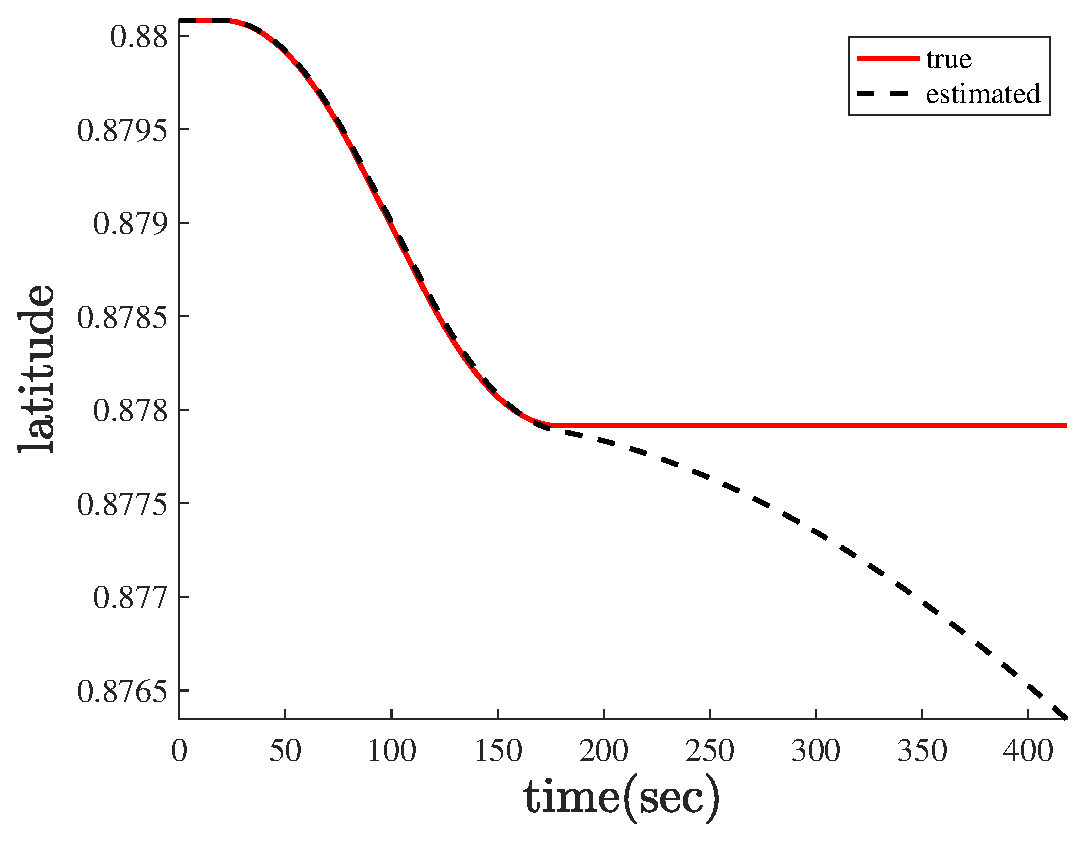
\includegraphics[width=0.7\textwidth]{../Figure/Q5/latitude_lin}
    \caption{Latitude}
\end{figure}
\begin{figure}[H]
    \centering
    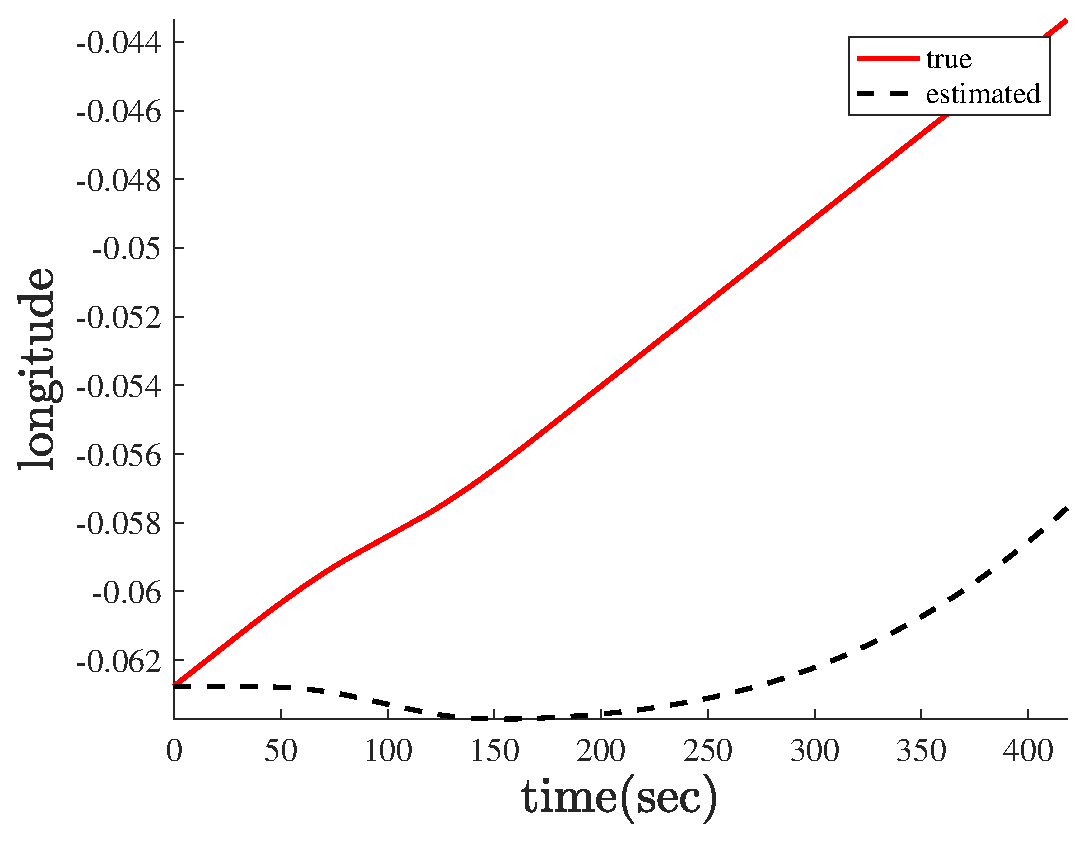
\includegraphics[width=0.7\textwidth]{../Figure/Q5/longitude_lin}
    \caption{Longitude}
\end{figure}
\begin{figure}[H]
    \centering
    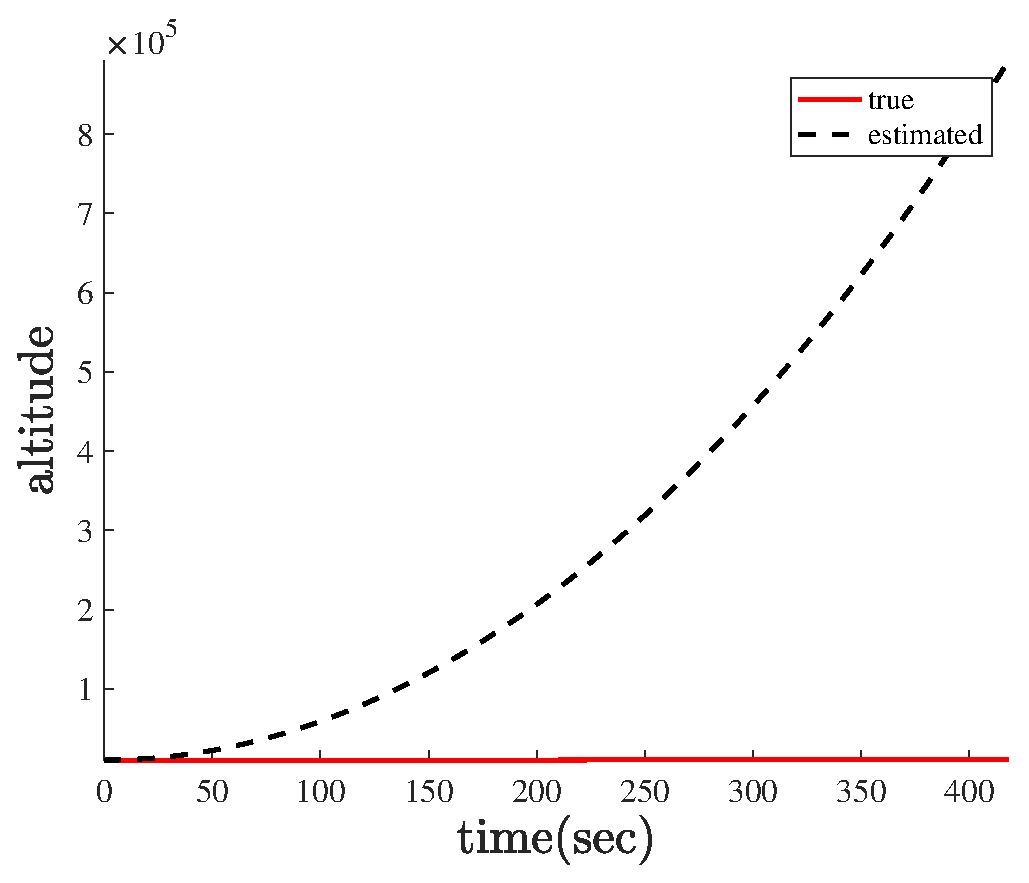
\includegraphics[width=0.7\textwidth]{../Figure/Q5/altitude_lin}
    \caption{Altitude}
\end{figure}
\begin{figure}[H]
    \centering
    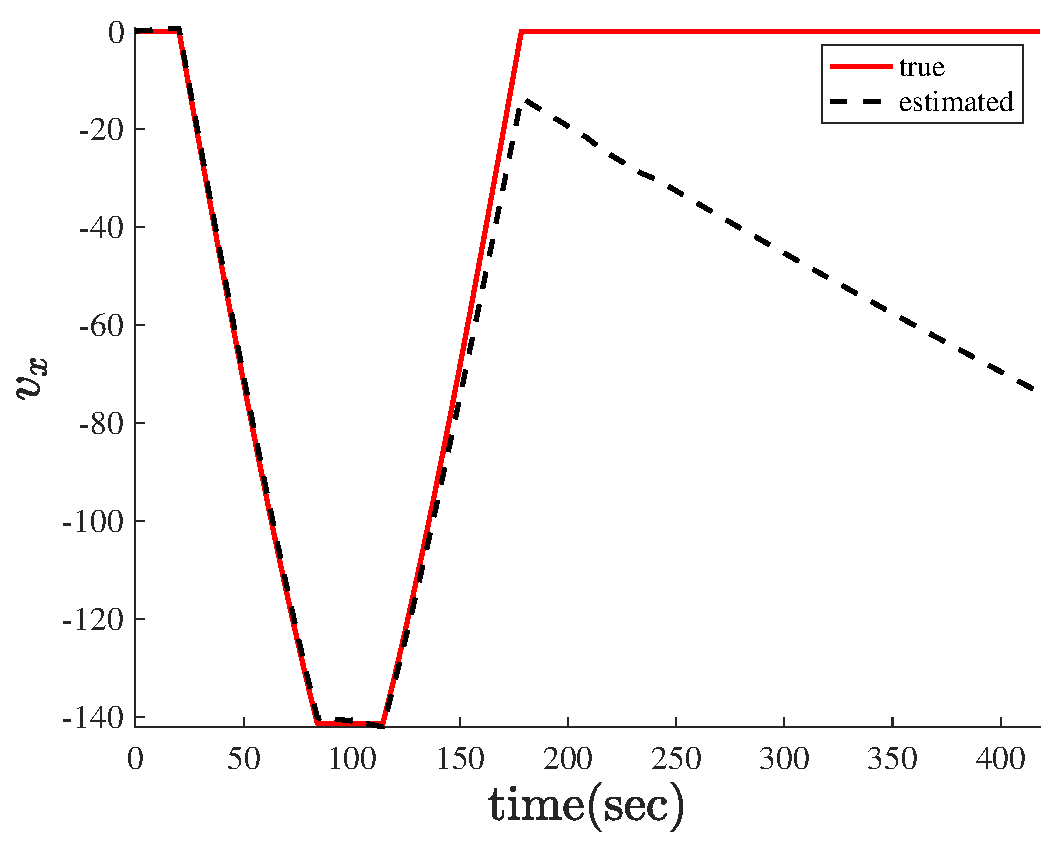
\includegraphics[width=0.7\textwidth]{../Figure/Q5/velocity_x_lin}
    \caption{Velocity in x direction}
\end{figure}
\begin{figure}[H]
    \centering
    \includegraphics[width=0.7\textwidth]{../Figure/Q5/velocity_y_lin}
    \caption{Velocity in y direction}
\end{figure}
\begin{figure}[H]
    \centering
    \includegraphics[width=0.7\textwidth]{../Figure/Q5/velocity_z_lin}
    \caption{Velocity in z direction}
\end{figure}

\begin{figure}
    \centering
    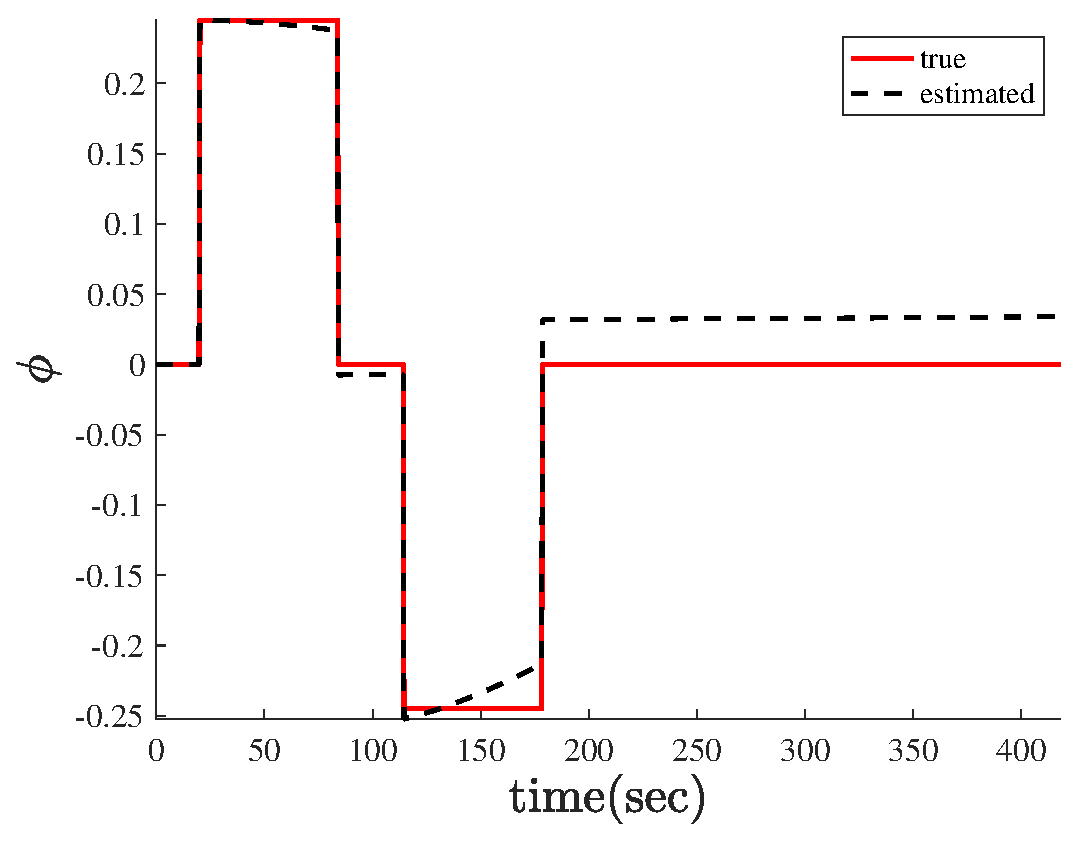
\includegraphics[width=0.7\textwidth]{../Figure/Q5/phi_lin}
    \caption{Roll}
\end{figure}
\begin{figure}
    \centering
    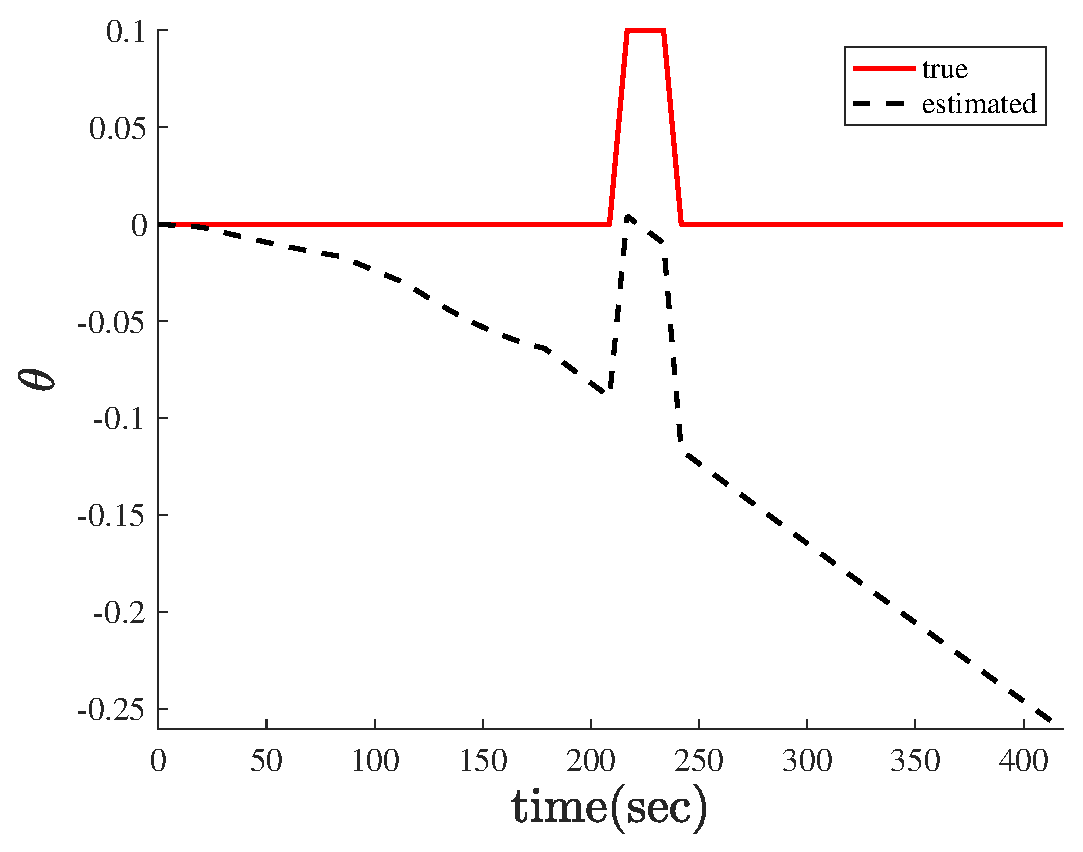
\includegraphics[width=0.7\textwidth]{../Figure/Q5/theta_lin}
    \caption{Pitch}
\end{figure}
\begin{figure}
    \centering
    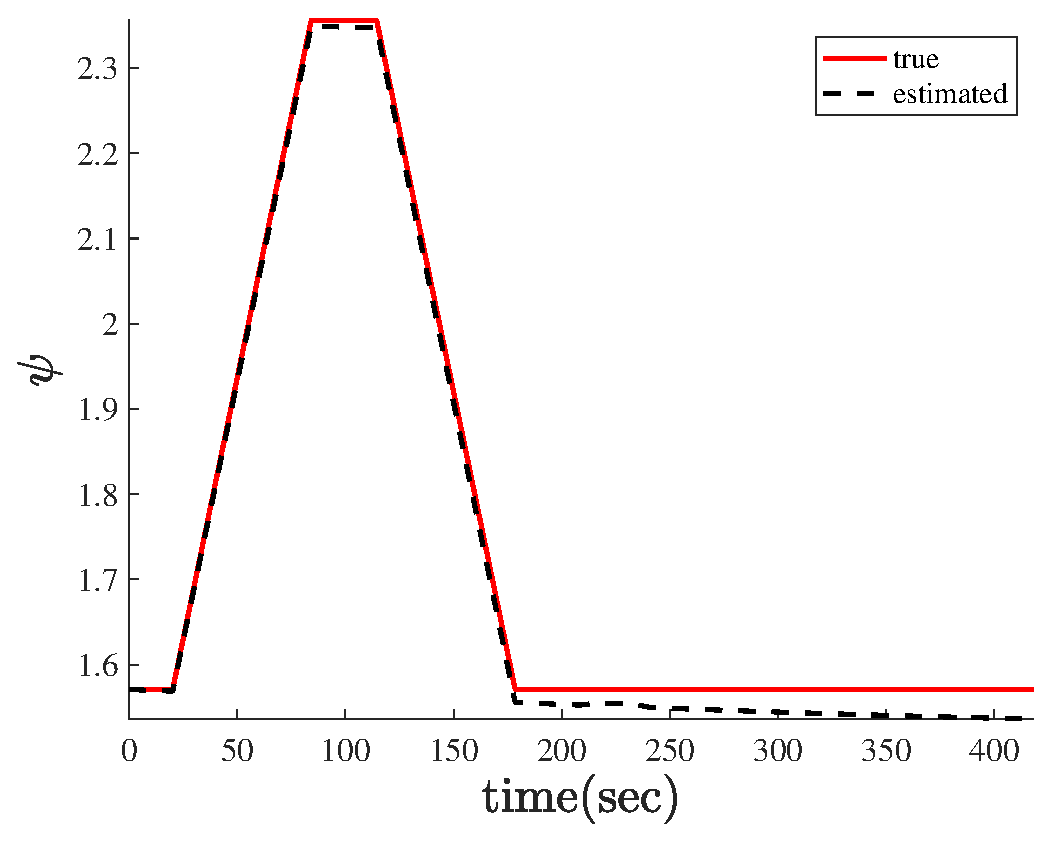
\includegraphics[width=0.7\textwidth]{../Figure/Q5/psi_lin}
    \caption{Yaw}
\end{figure}

